\label{Durchführung}

Sie befinden sich im Hauptmenü und möchten eine neue Messung starten.
\begin{itemize}
	\item Wählen und bestätigen Sie dazu im Hauptmenü den Punkt <Start new Measurement>.	
\end{itemize}

\begin{figure}[!hbt]
	\centering
	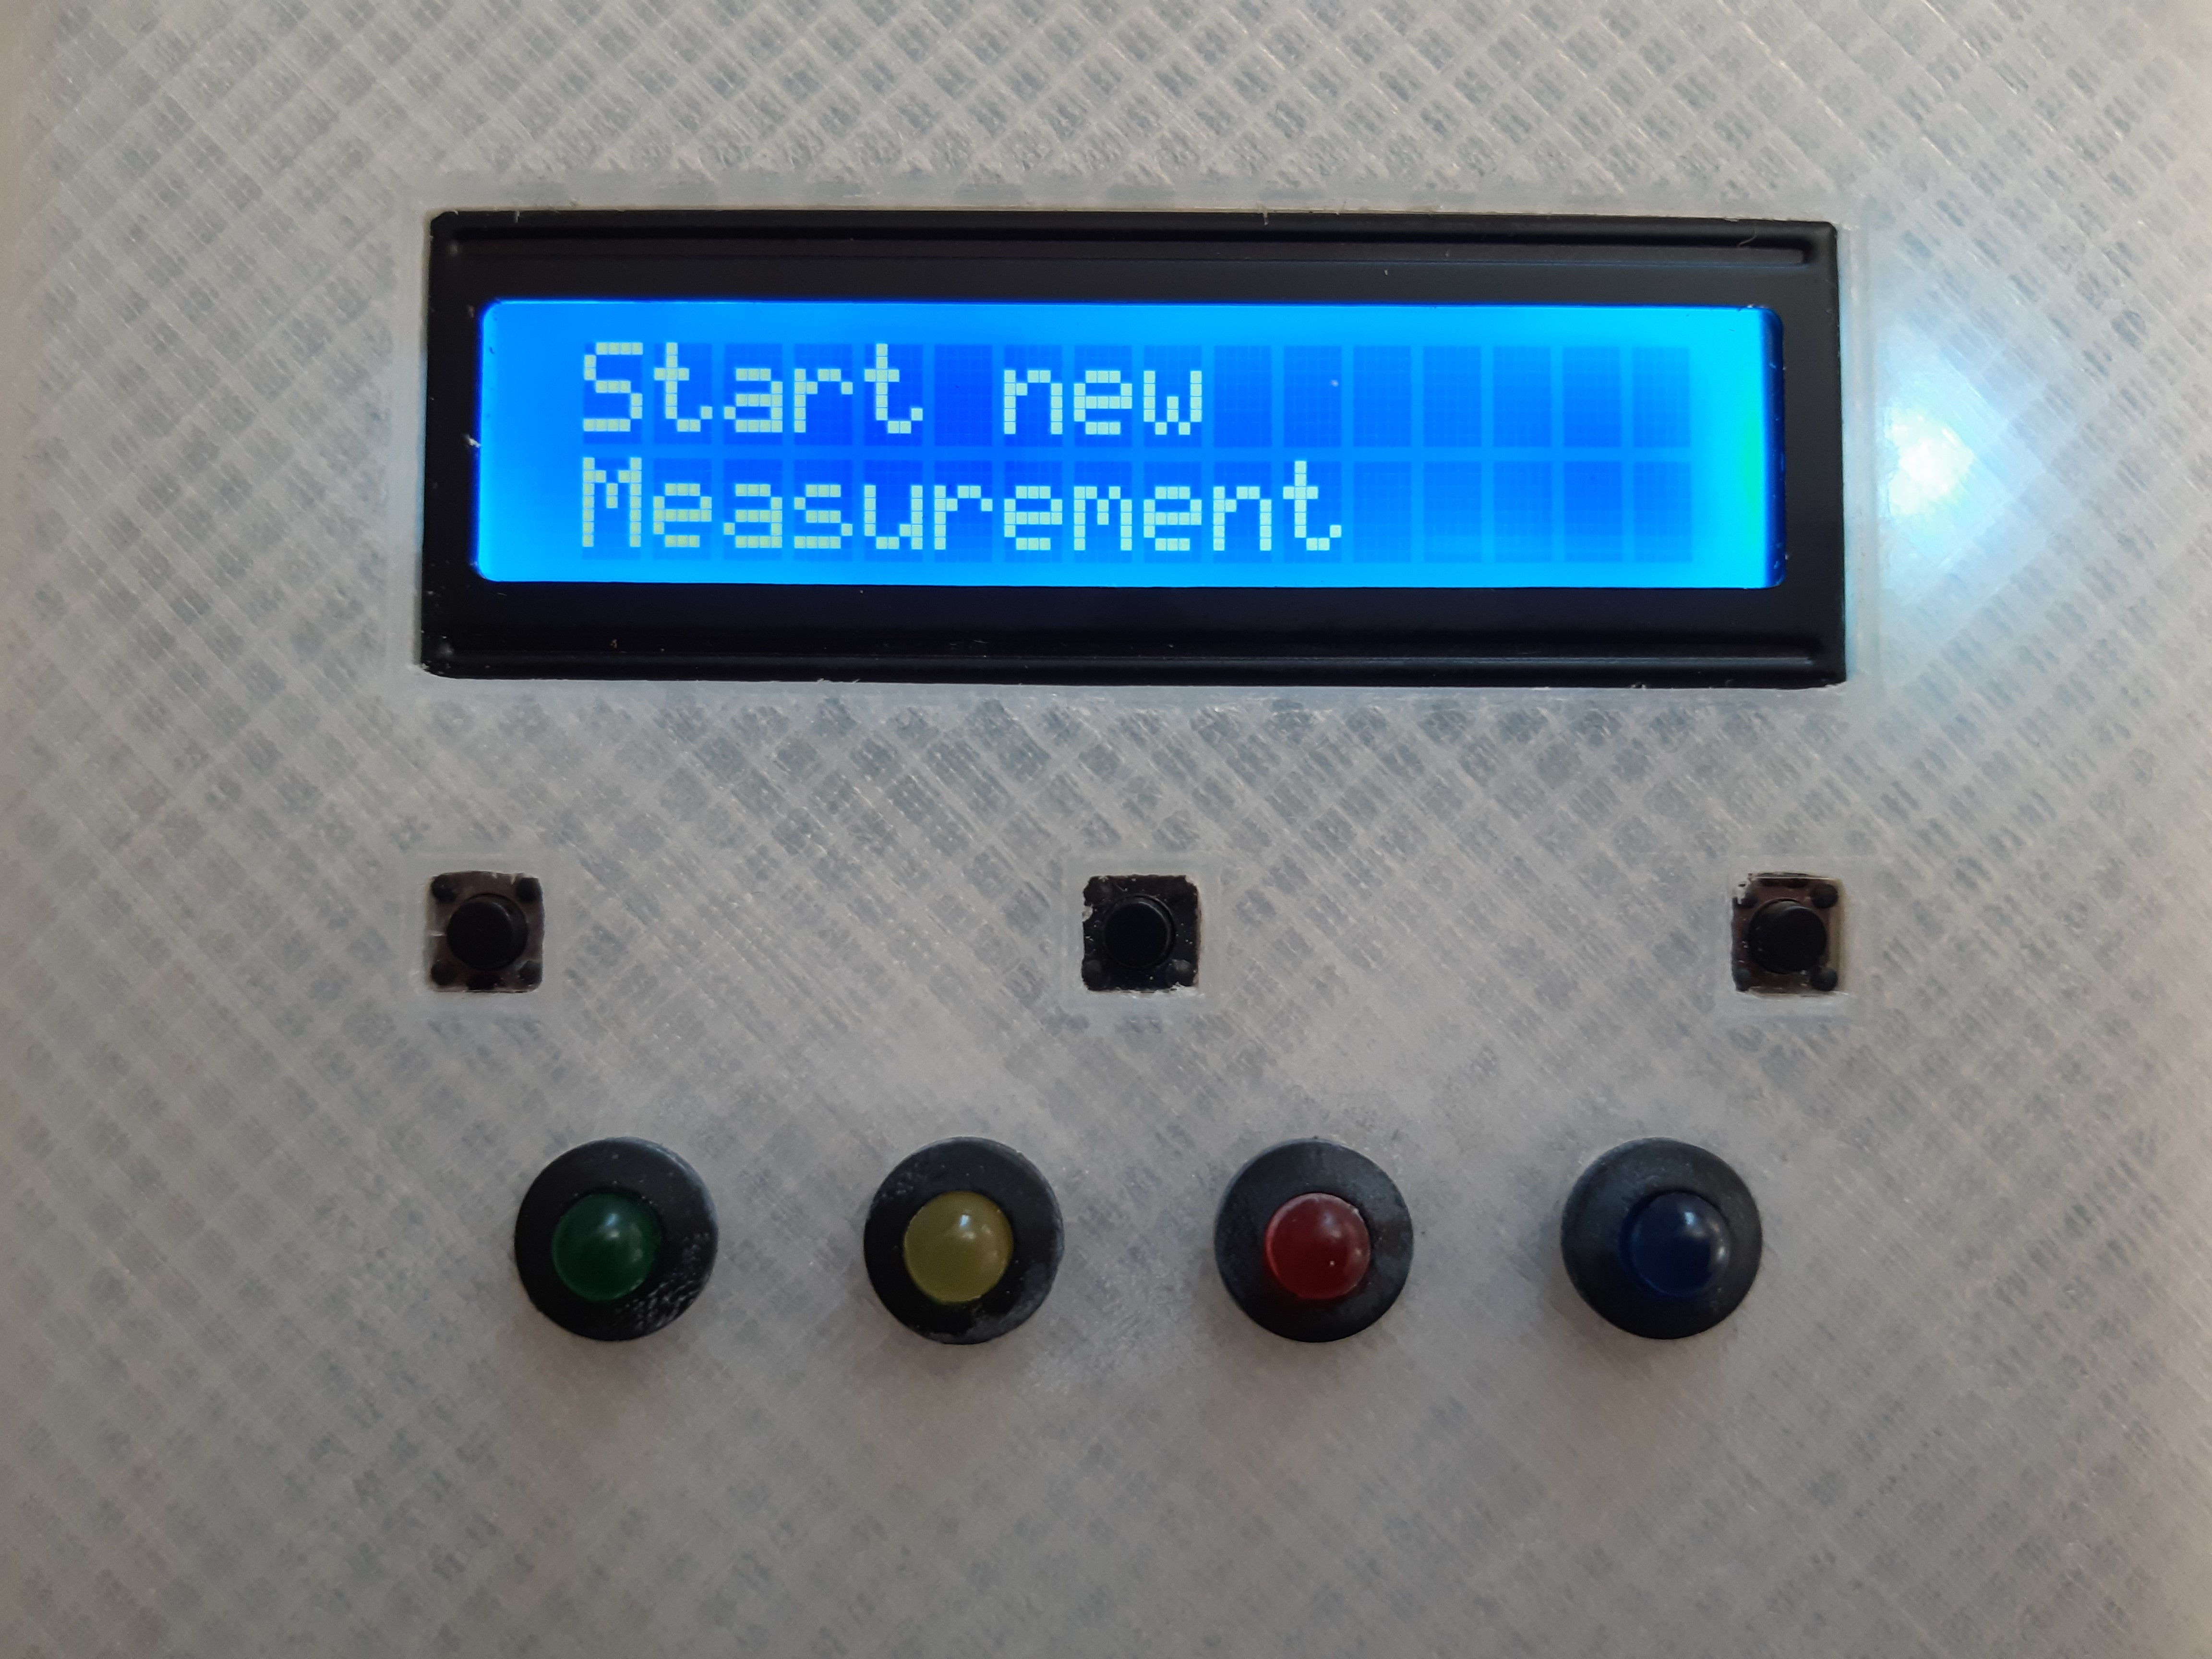
\includegraphics[width=0.4\linewidth]{Images/StartNewMeasurement}
	\footnotesize \\Quelle: eigene Aufnahme
	\caption{Hauptmenü: <Start new Measurement>}
	\label{fig:startnew}
\end{figure}

Anschließend können Sie zwischen drei Messmodi wählen.
\begin{itemize}
	\item Wählen und bestätigen Sie im angezeigten Menü den Messmodus, in welchem Sie verfahren möchten.	
\end{itemize}
Nach erfolgreichem Abschluss der Messung, kehren Sie in das Hauptmenü wieder zurück.

